\section{Eruptive Solar Flares}
\subsection{An Introduction to the Standard Eruptive Flare Model} 

Solar flares are the manifestation of magnetic energy release in the form of electromagnetic radiation spanning a wide range of wavelengths. These events are the most energetic phenomena associated with the Sun, with some of the larger flares releasing $10^{37}$ erg of energy. Flares are classified by the X-ray flux measured by the Geostationary Operational Environmental Satellite (GOES) see Table \ref{goes} below. \\

\begin{table}[h]
\centering
\begin{tabular}{|c|c|}\label{GOES}
Classification & Peak Flux Range at $1$ to $8\AA$ ($W.m^{-2}$)\\ 
\hline
X & $10^{-3}$ - $10^{-4}$\\ 
M & $10^{-4}$ - $10^{-5}$\\ 
C & $10^{-5}$ - $10^{-6}$\\ 
B & $10^{-6}$ - $10^{-7}$\\ 
A & $<10^{-7}$\\  
\end{tabular}
\caption{shows the GOES flare classification, which is based on powers of ten of hard x-ray flux. X class flares are the most powerful and A class are the weakest.}\label{goes}
\end{table}

The exact physical process governing the mechanics of solar flares is not known, however, magnetic reconnection is the currently accepted mechanism. Coronal magnetic loops tethered to sunspots of opposing polarity in the photosphere and sub-photosphere are twisted and stressed by movements of active regions across the solar surface. This shearing of the magnetic field, effectively stores energy as magnetic tension which can be released when opposing field lines meet and reconnect. The process of energy conversion is basically an unstable tensioned magnetic field relaxing back to a more stable configuration. As a result stored magnetic energy is converted to radiation, kinetic and thermal energy. The standard 2D flare model is the culmination of research by many authors,\citep{1964NASSP..50..451C, 1966Natur.211..695S, 1974SoPh...34..323H, 1976SoPh...50...85K}, and is still an ongoing area of research that is not entirely understood \citep{2011LRSP....8....6S}. In an active region, a closed magnetic field harbouring a prominence suddenly opens. As a result, plasma flows from the chromosphere to the corona. Because material in the chromosphere is denser than in the corona, flowing plasma experiences a drop in plasma pressure and an increase in magnetic pressure. This leads to reconnection of the open magnetic field lines, forming new loops at lower altitudes. Reconnection causes excess heating at the peaks of newly connected loops which conducts down toward the chromosphere. Also, particles are accelerated by the new magnetic configuration, flowing to the chromosphere. This injection of thermal energy and accelerated particles heats the chromosphere causing HXR footpoints \citep{1995ApJ...455..347A} and UV ribbons \citep{2009A&A...493..241F}. As a result, some chromospheric material evaporates upward into newly created flare loops, whilst some material propagates downward toward the lower chromosphere, known as condensation. The flare loop cools and the process starts again in the next consecutive loop until the unstable magnetic field has relaxed to a state that is closer to it's stable,  potential state. In eruptive flares, energy is released every time a new reconnection of a neighbouring loop occurs, this said to be the reason that flare ribbons move away from each other as the flare evolves. \\
White light flares are said to be rare events only associated with the most energetic of solar flares, they occur when flare energy is transported deep into the dense lower atmosphere causing an enhancement in optical wavelengths. It is thought this happens due to an energetic particle beam transporting energy to the lower atmosphere where it's energy dissipates into the dense chromospheric or photospheric material. The collisional thick target model by \cite{1971SoPh...18..489B} says that almost all of the flare energy is carried by the particle beam, therefore, energy dissipated in the lower atmosphere represents a large portion of the flare energy budget. White light enhancement from the lower atmosphere can be explained by either, Balmer \& Paschen continuum emission from the chromosphere caused by hydrogen recombination or direct photospheric heating \citep{2007ASPC..368..417D} by radiative backwarming \citep{1989SoPh..124..303M}. 


\begin{figure}[H]
  \begin{center}
  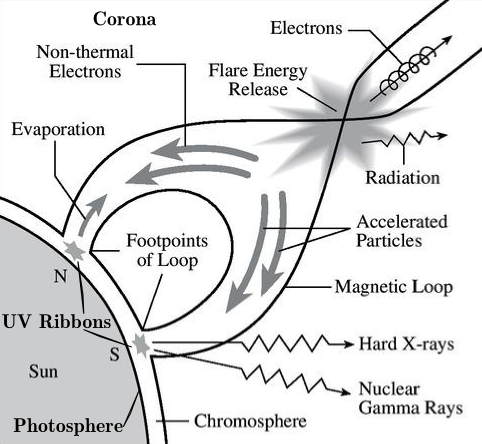
\includegraphics[width=0.40\textwidth]{flare}
  \caption{cartoon of the standard 2D solar flare model.}\label{flare-cartoon}
\end{center}
\end{figure}


%It is also theoretically possible to heat the upper photosphere by resistive dissipation of Alfven waves \citep{1982SoPh...80...99E}


\subsubsection{Solar Atmosphere}
The solar atmosphere \citep{2003dysu.book.....D, 2004soas.book.....F} is described as having four main components, the corona, transition region, chromosphere and photosphere, see \ref{solatmpics}. 

\begin{figure}[H]%\label{sunquake-cartoon}
  \begin{center}
  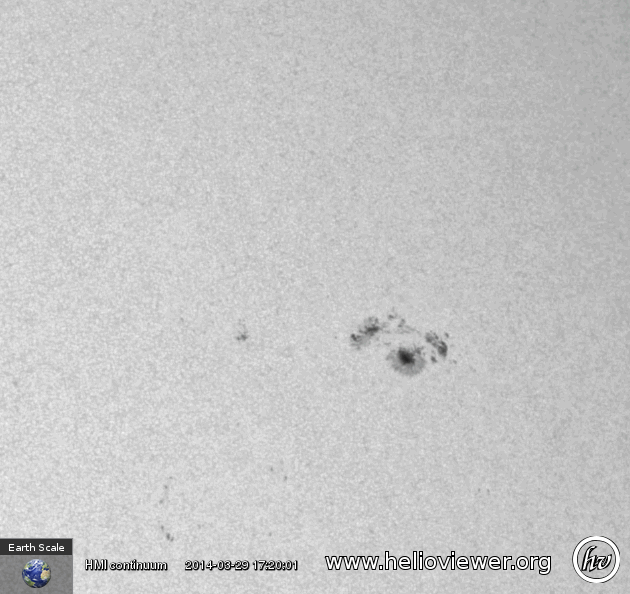
\includegraphics[width=0.20\textwidth]{2014_03_29_17_19_42_HMI_Int}%photsphere
  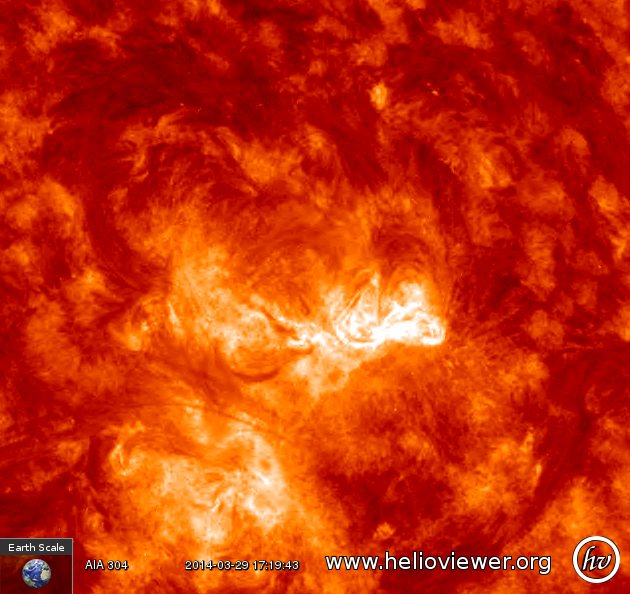
\includegraphics[width=0.20\textwidth]{2014_03_29_17_19_42_AIA_304}%chromosphere
  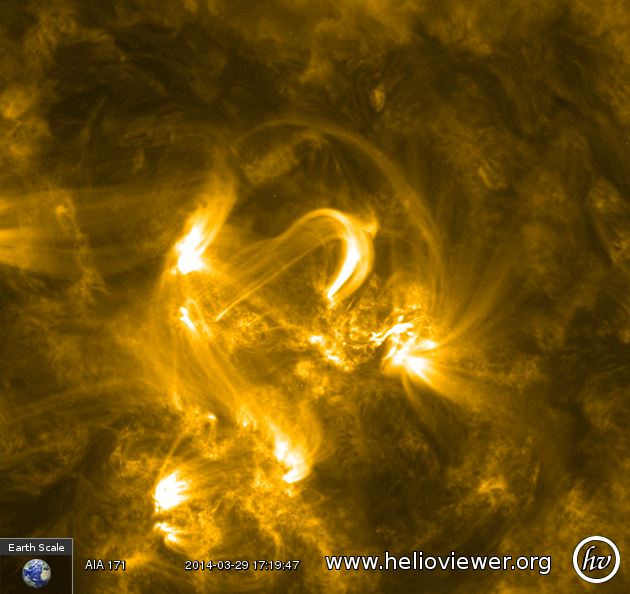
\includegraphics[width=0.20\textwidth]{2014_03_29_17_19_42_AIA_171}%tr
  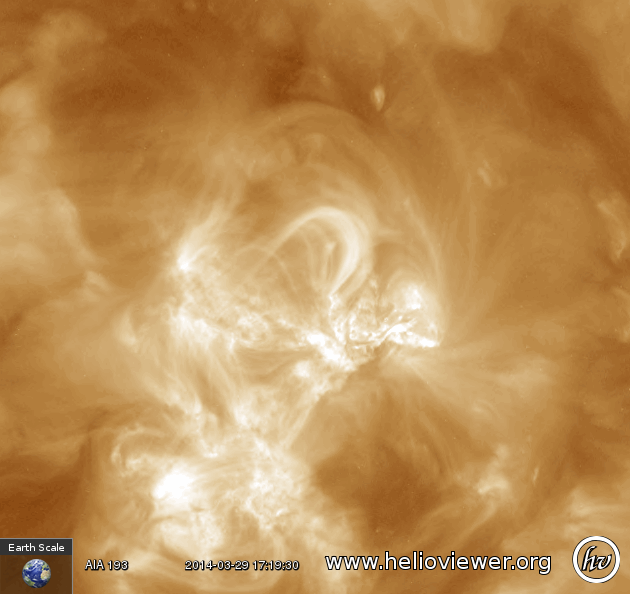
\includegraphics[width=0.20\textwidth]{2014_03_29_17_19_42_AIA_193}%corona
  \caption{ Images taken from the Solar Dynamics Observatory (SDO) instruments, the Helioseismic Magnetic Imager(HMI) and the Atmospheric Imaging Assembly (AIA) displaying the four main components of the solar atmosphere. From left to right layers of the solar atmosphere are increasing in altitude and temperature from the photosphere (SDO/HMI $6173\AA$ continuum), to the chromosphere (SDO/AIA $304\AA$) through the transition region (SDO/AIA $171\AA$) then up to the corona (SDO/AIA $193\AA$).}\label{solatmpics}
\end{center}
\end{figure}


For a sunquake to occur, energy released during a solar flare has to traverse these four layers propagating through nine pressure scale heights as it does so. Pressure scale height is a measure of the distance over which pressure drops off by a factor of $\exp$), 


for example, in the photosphere, $H\sim150$km, whereas in the corona, $H\sim100$Mm. The photosphere where sunquakes form observable wavefronts and is the lowest in altitude of the four layers characterised. With an effective temperature of $T=5800$K, the photosphere decreases in temperature with radial distance. Due to the assumption that this region emits as a black body the temperature is estimated using Wien's displacement law. If white light enhancement is observed in the photosphere, it is thought to be an indicator of the \textbf{Radiative backwarming} progenitor of sunquake generation, which can also be a bi-product caused by both the \textbf{Shocks} and \textbf{Direct proton collision} progenitors. The plasma beta (a measure of the ratio between gas and magnetic pressure) in this region is mostly larger than one $\beta >1$ meaning plasma pressure is dominant in dictating plasma motions, the exception to this exists in sunspots where $\beta<1$ and magnetic pressure is dominant. \\ 

Found in active regions of the photosphere, sunspots are regions of intense magnetic field playing host to footpoints of loops that can extend out into interplanetary space. They are made up of two main parts, the dark central umbra, surrounded by the slightly less dark penumbra. The umbra hosts magnetic field lines that are tightly packed and pointing radially away from the Sun, whereas the penumbral magnetic field is more horizontal. During a solar flare, coronal loops reconnect causing a reconfiguration of the magnetic field tethered at sunspot locations, at this point, penumbral field lines can collapse toward the photosphere, imparting a Lorentz force on local plasma. This leads to the \textbf{Sudden magnetic field reconfiguration} progenitor of sunquake generation. Other features that are part of the photosphere include granules and super granules (seen only in Doppler images), which are the physical representation of convection currents. Heated plasma rises from below the surface and is seen as the bright central part of the granule, the darker surrounding regions are cooler material sinking back into the interior. \\

The next region of the atmosphere is the chromosphere which is situated above the photosphere. This layer of plasma is a few thousand kilometres (2000-3000km) thick and is optically thin to visible light so is difficult to see against the brightness of the photosphere. The temperature in this layer increases with height and ranges from 4400K at the temperature minimum region to $\sim10^{5}$K at the top, as a result, $\beta$ drops rapidly crossing unity as it does so. The pressure scale height in this region is changing with altitude. The dominant emission in this region is H$\alpha$ at $6563\AA$.Through the transition region to the corona and the atmosphere starts to heat considerably to $T\sim10^{7}$K. This region is visible in white light due to Thompson scattering of photospheric light by free electrons and dust in the coronal magnetic field. The plasma beta is less than one through the entire corona meaning magnetic forces dominate. Figure \ref{solatm} shows how the solar atmosphere changes with height, temperature and density, giving an indication of the stratification of atmospheric layers.

\begin{figure}[H]
  \begin{center}
    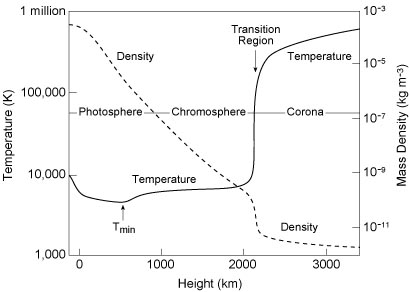
\includegraphics[width=0.6\textwidth]{solar-atm-plot}
\caption{The temperature of the solar atmosphere decreases from values near 6,000 degrees Kelvin at the visible photosphere to a minimum value of roughly 4,400 degrees Kelvin about 500 kilometers higher up. The temperature increases with height, slowly at first, then extremely rapidly in the narrow transition region, less than 100 kilometers thick, between the chromosphere and corona, from about $10^{4}$K to about $10^{6}$K. (Courtesy of Eugene Avrett, Smithsonian Astrophysical Observatory.)}\label{solatm}
  \end{center}
\end{figure}

  
\subsection{Observing Solar Flares}
Using data collected by spacecraft observing the Sun, energy released during solar flares can be tracked as it is deposited throughout the atmosphere. 

Energy deposition in the corona and upper chromosphere is marked by HXR footpoints and UV ribbons. The Ramaty High Energy Solar Spectroscopic Imager (RHESSI) observes solar emission ranging from X-rays to $\gamma$-rays produced by energetic particles and nuclear interactions. RHESSI was designed with the aim of understanding impulsive energy release, particle acceleration and transportation in the magnetohydrodynamic environment of the solar atmosphere. Using 25 - 50 keV and 50 - 100 keV intensity data collected by RHESSI, HXR footpoints can be tracked and analysed. Observing UV ribbons requires a different spacecraft. The Interface Region Spectroscopic Imager (IRIS) captures near-ultraviolet (NUV) and far-ultraviolet (FUV) emission and is designed to observe the chromosphere at various altitudes. Emission is collected by a slit-jaw imager (SJI) and a spectrometer (SG) simultaneously. The spectrograph is sensitive in both FUV and NUV passbands, which expose 3 CCDs to produce spectra in three UV bands, two FUV and one NUV. Table \ref{iris-sg} shows how each passband relates to emission processes occurring from the upper-chromosphere down to the upper-photosphere. 

\begin{table}
\centering
\begin{tabular}{|c|c|c|c|}
Band & Wavelength $\AA$ & Temperature $\log{T}$ & Region of Atmosphere\\ 
\hline
FUV 1 & $1331.7 - 1358.4$ & $3.7 - 7.0$ & Upper to lower-chromosphere\\ 
FUV 2 & $1389.0 - 1407.0$ & $3.7 - 5.2$ & Upper to lower-chromosphere\\ 
NUV & $2782.7 - 2851.1$ & $3.7 - 4.2$ & Chromosphere to upper-photosphere\\ 
\end{tabular}
\caption{The IRIS/SG is capable of observing three passbands, which relate to different plasma temperatures.}\label{iris-sg}
\end{table}

The slit-jaw images, are light collected from a reflective area surrounding the slit. The imager is capable of observing four wavelengths relating to emission at different altitudes as shown by table \ref{iris-sj}. 

\begin{table}
\centering
\begin{tabular}{|c|c|c|c|c|}
SJI Passband & Wavelength $\AA$ & FWHM $\AA$ & Temperature $\log{T}$ & Region of Atmosphere\\ 
\hline
C II  & $1330$ & $40$ & $3.7 - 7.0$ & Upper-chromosphere\\ 
Si IV  & $1400$ & $40$ & $3.7 - 5.2$ & Upper-chromosphere\\ 
Mg II h/k & $2796$ & $4$ & $3.7 - 4.2$ & Lower-chromosphere\\ 
Mg II wing & $2832$ & $4$ & $3.7 - 3.8$ & Upper-photosphere\\   
\end{tabular}
\caption{The IRIS/SJ is capable of observing four passbands, which relate to different plasma temperatures.}\label{iris-sj}
\end{table}  

Signatures from energy deposition in the lowest regions of atmosphere are captured by Solar Dymanics Observatory's (SDO) Helioseismic Imager (HMI), which observes the photosphere. Able to observe optical continuum intensity (6173Å), Helioseismic and magnetic data SDO/HMI can provide valuable data concerning WLFs, sunquakes and magnetic field configuration. Optical continuum data can provide information about WLFs and radiative backwarming of photospheric material, which is a possible sunquake progenitor. Helioseismic data can be used to analyse the movement of material during a solar flare, such as downward flows which could indicate shocks propagating from higher altitudes or particle beams penetrating the atmosphere. The point of origin and wavefronts of a sunquake can also be detected using helioseismic data, which can be used to calculate acoustic power of the quake. Magnetic data from SDO/HMI shows local magnetic field direction, useful for determining the presence of impulsive changes in magnetic field capable of generating a sunquake.     




